\documentclass[12pt]{article}


% --- math/fonts ---
\usepackage{amsmath,amssymb}
\usepackage{braket}
\usepackage[T1]{fontenc}
\usepackage{libertine}
\usepackage[utf8]{inputenc}

% --- graphics/tikz ---
\usepackage{tikz}
\usepackage{qcircuit}

% --- other stuff ---
\usepackage[margin=1in]{geometry}
\usepackage{pdfpages}
\usepackage{multicol}
\usepackage[shortlabels]{enumitem}
\usepackage{cancel}
\usepackage{graphicx}
\usepackage{float}
\usepackage{listings}
\lstset{
    language=Python,
    basicstyle=\ttfamily\footnotesize,
    keywordstyle=\bfseries,
    frame=single,
    breaklines=true,
    keepspaces=true,
    columns=fullflexible,
    showstringspaces=false
}
\let\epsilon\varepsilon
\usepackage{enumitem}
\setlist[enumerate]{label=\arabic*.}
\usepackage[authoryear,round]{natbib}
\usepackage[hidelinks]{hyperref}


\newcommand{\class}{CSCE883 Machine Learning}           
\newcommand{\examnum}{Homework 1}      
\newcommand{\examdate}{09/06/2026}        
\newcommand{\timelimit}{}             




\begin{document} 
\pagestyle{plain}
\thispagestyle{empty}

\noindent
\begin{tabular*}{\textwidth}{l @{\extracolsep{\fill}} r @{\extracolsep{6pt}} l}
 \textbf{\class} & \textbf{Name:} & \textit{Taylor Belcher}\\       
\textbf{\examnum} &&\\
\textbf{\examdate} &&\\
\end{tabular*}\\
\rule[2ex]{\textwidth}{2pt}
% ---

 
\begin{enumerate}
    \item \emph{(Question 1)} The Jupyter notebook file \emph{Q1.ipynb} has all relevant code for this problem. Codex GPT-6 Astra assisted me in writing the code. After implementing 
    a basic euclidean distance function, I created a K-nearest neighbors classifier that used the provided training file to predict on the test file for $k=1 ... 9$. Note that in the definition
    of the knn\_clasifier, ties are decided by choosing the label of the nearest neighbor since the labels array is sorted by increasing distance from least to greatest, and the max would return the first label in the case of a tie.\\


\begin{lstlisting}
def euclidean_distance(dimension, point1, point2):
    squared_distance = 0
    for i in range(dimension):
        squared_distance += (point1[i] - point2[i]) ** 2
    return squared_distance ** 0.5


def knn_classifier(k, training_data, test_point):
    distances = []
    for data_point in training_data:
        distance = euclidean_distance(len(test_point), data_point[:-1], test_point)
        distances.append((distance, data_point[-1]))
    distances.sort(key=lambda x: x[0])
    k_nearest_neighbors = distances[:k]
    labels = [neighbor[1] for neighbor in k_nearest_neighbors]
    return max(labels, key=labels.count)
\end{lstlisting}

I got the following results, which are also in the notebook file:

\begin{center}
    \textbf{kNN results on the original, unscaled data}\par\smallskip
    \small
    \setlength{\tabcolsep}{3pt}
    \begin{tabular*}{\linewidth}{@{\extracolsep{\fill}}l*{9}{c}@{}}
        \hline
        $K$ & 1 & 2 & 3 & 4 & 5 & 6 & 7 & 8 & 9 \\
        \hline
        Correct predictions & 462 & 462 & 462 & 462 & 462 & 462 & 462 & 462 & 462 \\
        Accuracy & 1.000 & 1.000 & 1.000 & 1.000 & 1.000 & 1.000 & 1.000 & 1.000 & 1.000 \\
        \hline
    \end{tabular*}
\end{center}

I was surprised that the accuracy was 100\% for all $k$-values and I was concerned that I had implemented the algorithm incorrectly. But after reviewing my implementation, I think it is correct. 
Next, I implemented min-max normalization and standardization to scale the data and then re-ran my KNN algorithm. In both cases, if a certain feature in the training data had zero variance or was constant, I set that feature to 0. 



\newpage
\begin{lstlisting}[basicstyle=\ttfamily\fontsize{9}{10.5}\selectfont]
def min_max_normalize(data, feature_ranges=None):
    # When no ranges are supplied, calculate them from the training data.
    if feature_ranges is None:
        feature_ranges = []
        for i in range(len(data[0]) - 1):  # Exclude the final label column.
            column = [row[i] for row in data]
            feature_ranges.append((min(column), max(column)))

    normalized_data = []
    for row in data:
        normalized_row = []
        for i in range(len(row) - 1):
            min_value, max_value = feature_ranges[i]
            if max_value == min_value:
                normalized_value = 0.0  # Ignore a constant training feature.
            else:
                normalized_value = (row[i] - min_value) / (max_value - min_value)
            normalized_row.append(normalized_value)
        normalized_row.append(row[-1])  # Keep the original class label.
        normalized_data.append(normalized_row)

    return normalized_data, feature_ranges
\end{lstlisting}

\begin{lstlisting}[basicstyle=\ttfamily\fontsize{9}{10.5}\selectfont]
def standardize(data, feature_stats=None):
    # When no stats are supplied, calculate them from the training data.
    if feature_stats is None:
        feature_stats = []
        for i in range(len(data[0]) - 1):  # Exclude the final label column.
            column = [row[i] for row in data]
            mean = sum(column) / len(column)
            variance = sum((x - mean) ** 2 for x in column) / len(column)
            std_dev = variance ** 0.5
            feature_stats.append((mean, std_dev))

    standardized_data = []
    for row in data:
        standardized_row = []
        for i in range(len(row) - 1):
            mean, std_dev = feature_stats[i]
            if std_dev == 0:
                standardized_value = 0.0  # Ignore a constant training feature.
            else:
                standardized_value = (row[i] - mean) / std_dev
            standardized_row.append(standardized_value)
        standardized_row.append(row[-1])  # Keep the original class label.
        standardized_data.append(standardized_row)

    return standardized_data, feature_stats
\end{lstlisting} 

I re-ran the KNN classifer on the two versions of the scaled data and got the following results: 

\begin{center}
    \begin{minipage}{\linewidth}
    \centering
    \textbf{Min--max normalization}\par\smallskip
    \small
    \setlength{\tabcolsep}{3pt}
    \renewcommand{\arraystretch}{1.2}
    \begin{tabular*}{\linewidth}{@{\extracolsep{\fill}}l*{9}{c}@{}}
        \hline
        $K$ & 1 & 2 & 3 & 4 & 5 & 6 & 7 & 8 & 9 \\
        \hline
        Correct predictions & 461 & 461 & 461 & 461 & 461 & 461 & 461 & 461 & 461 \\
        Accuracy & 0.998 & 0.998 & 0.998 & 0.998 & 0.998 & 0.998 & 0.998 & 0.998 & 0.998 \\
        \hline
    \end{tabular*}
    \end{minipage}
\end{center}

\begin{center}
    \begin{minipage}{\linewidth}
    \centering
    \textbf{Standardization}\par\smallskip
    \small
    \setlength{\tabcolsep}{3pt}
    \renewcommand{\arraystretch}{1.2}
    \begin{tabular*}{\linewidth}{@{\extracolsep{\fill}}l*{9}{c}@{}}
        \hline
        $K$ & 1 & 2 & 3 & 4 & 5 & 6 & 7 & 8 & 9 \\
        \hline
        Correct predictions & 461 & 461 & 461 & 461 & 461 & 461 & 461 & 461 & 461 \\
        Accuracy & 0.998 & 0.998 & 0.998 & 0.998 & 0.998 & 0.998 & 0.998 & 0.998 & 0.998 \\
        \hline
    \end{tabular*}
    \end{minipage}
\end{center} 

Both scaling methods resulted in a slight decrease in accuracy, misclassifying only one test point. I was again suprised because I had expected that scaling would only 
improve accuracy, or at least not hurt it. Given that the original data had perfect accuracy, I thought the scaled versions would also. I was again worried that I had implemented the algorithm incorrectly, but I cannot identify what is wrong with the implementation so 
I am working on the assumption that the given data has been set up this way on purpose and that my implementation is correct. 

Given these results, it would appear that the original unscaled data is the best approach for this particular dataset, but that is not necessarily true in general. I wanted to know which
point was misclassified, so the additional code in the file was created by Codex to help me identify which point label was changed after scaling. 

In general, I would expect scaling to improve accuracy for the KNN algorithm so that no one feature has an outsized influence on the calcuated distance, but if one feature already has low variance, 
it's change from the original data to scaling might mean that after scaling it can influence the classification. Feature 4 from the csv appears to do that in this case. I became curious about whether
we could drop a feature entirely and still perfectly predict the test set. I prompted Codex to check all possible subsets of the features and run the KNN algorithm for the original data and the two different
scaled data. This code showed that if we dropped Feature 4 and used the standardized data, we could stil get 100\% accuracy for $k=1 ... 9$. I think this supports my hypothesis that Feature 4 is the one that is causing the misclassification after scaling.

\item \emph{(Question 2)} 
These summaries are written by me. I asked for feedback from Codex on what I wrote and made some edits based on AI feedback, but I am the author. 

The first paper that I read was \emph{Deep Nearest Neighbor Anomaly Detection} by \cite{bergman2020deep}. The paper proposes and tests using an available neural network image classifier to first extract features of the image and then perform kNN on the extracted features to detect anomalous images. They call it Deep Nearest Neighbors (DN2).
Identifying anomalous images is advantageous in threat assessment and preventative maintenance. For example, a stream monitoring an oil pipeline might be able to detect evidence of corrosion and immiment failure. Anomaly detection training can be \emph{supervised, semi-supervised,} or emph{unsupervised}. In particular,
they were interested in the \emph{semi-supervised} cases where the training set has no anomalous images and \emph{unsupervised} cases where unlabeled normal and anomalous images are in the training set. The authors ran the ImageNet pre-trained ResNet feature extractor on both the training and test images. The authors note that
the majority of training time comes from neural net inference to extract features and that more layers produces better results, but that DN2 is able to perform well even with a very small training set, as evidenced by their figure showing average ROC area. They also investigated identifying groups of images rather than single images, but noted that 
larger groups makes the task more difficult. They also noted that kNN time increases with larger datasets, but they suggested first doing k-means and then performing kNN on the cluster centers to reduce the number of comparisons. Besides time to classification increasing with large data sets, the authors noted that the pretrained features might be less effective on images
very dissimilar to those in ImageNet. 

\begin{figure}[H]
    \centering
    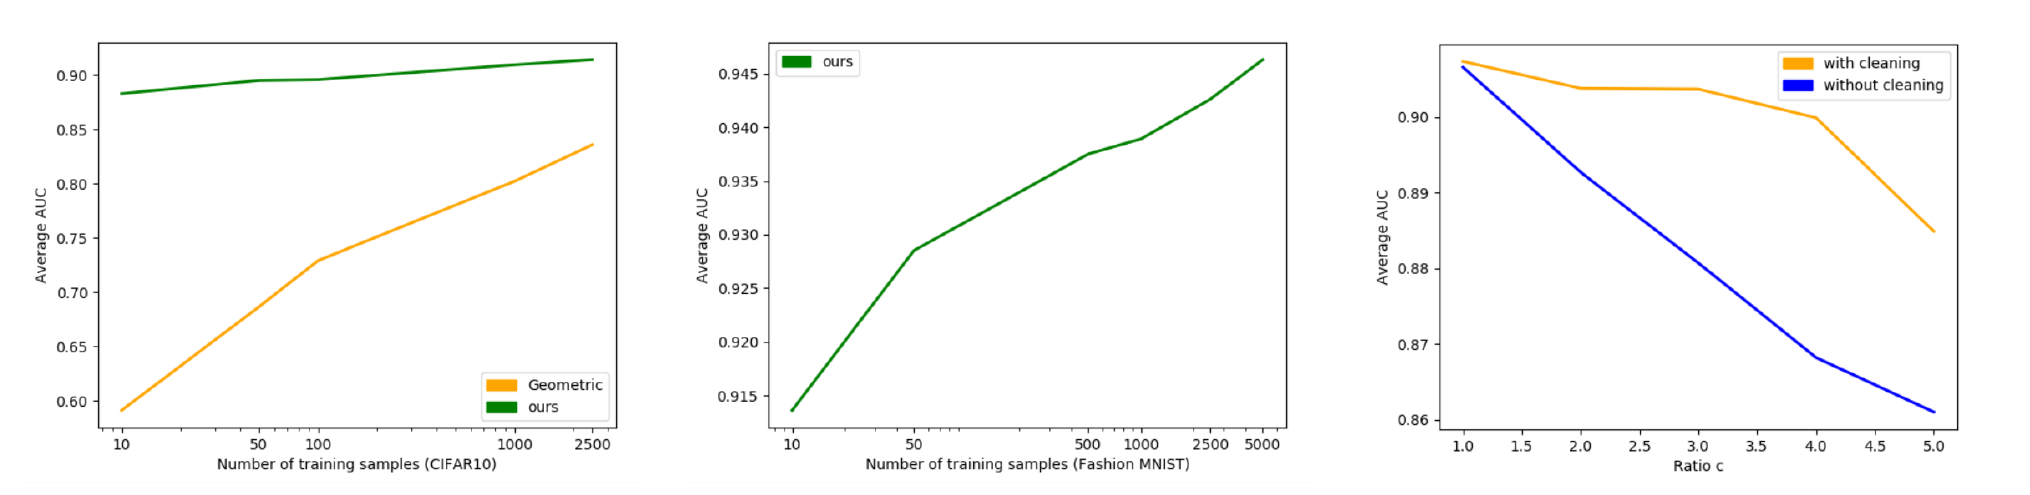
\includegraphics[width=\linewidth]{figures/bergman2020-figure5.png}
    \caption{Reproduced from Figure 5 of \citet{bergman2020deep}.}
    \label{fig:bergman-figure5}
\end{figure}

This idea of reducing the size of the training set in particular stood out to me. Cluster centers make sense as a representative reduction of a larger set, but I am curious if we not just place the rough location of a test point
and then just test the values within a ball of a given radius of that test point rather than comparing to the entire training corpus. Perhaps an algorithm that could quickly place the test point in an approximate 
``quadrant'' of available training data and then only compare to the training points in that quadrant. If the training data was already processed, not unlike k-means clustering, then we could already know a subset of training data points that are near a given training data point. Specifying the algorithm for grouping the training points and comparing it's 
speed and accuracy to k-means clustering and then kNN on the cluster centers would be one way to test this idea. Codex tells me that my idea is close to the kd-trees mentioned in the paper. 

\clearpage
The second paper I read was \emph{Deep k-Nearest Neighbors: Towards Confident, Interpretable and Robust Deep Learning} by \cite{papernot2018deep}. While the previous paper looked at using a neural network to first process images that could then be analyzed with k nearest neighbors, this paper attempts to improve neural network performance with the kNN algorithm. In particular,
the authors were interested in looking at the interpretability of a deep neural network at intermediate stages as well as improving the robustness of DNN models against adversarial attacks. Their idea was to perform kNN on each intermediate layer output to check how similar that output was to expected outputs for the training data. As they say in the paper, they wanted to answer ``Why did the model decide that?''. In the included figure from the paper,
you can see how they are using k nearest neighbors to check intermediate outputs from the neural network and see if they are conformal, that is, the match all through through the network during the hidden layers. 

Their results show that by checking intermediate outputs from the layers of the neural network and comparing them with kNN, their DkNN model has a higher accuracy because of lower credibility (it's estimate of the probability of correct classification) than traditional DNNs and is also more robust against adverarial attacks because of this lower credibility. They were even able to find mislabeled data in the MNIST data set
by searching for inputs with high credibility in the model but had been marked as incorrect predictions. The models also outperform softmax on out of training examples because they had low credibliity on the new data. The authors seem to think this approach is very strong, as the scenario they describe for a successful adversarial attack requires inside knowledge and would mean targeting an image that stays conformal within the intermediate stages of the DkNN despite ultimately being an anomalous image. 


\begin{figure}[H]
    \centering
    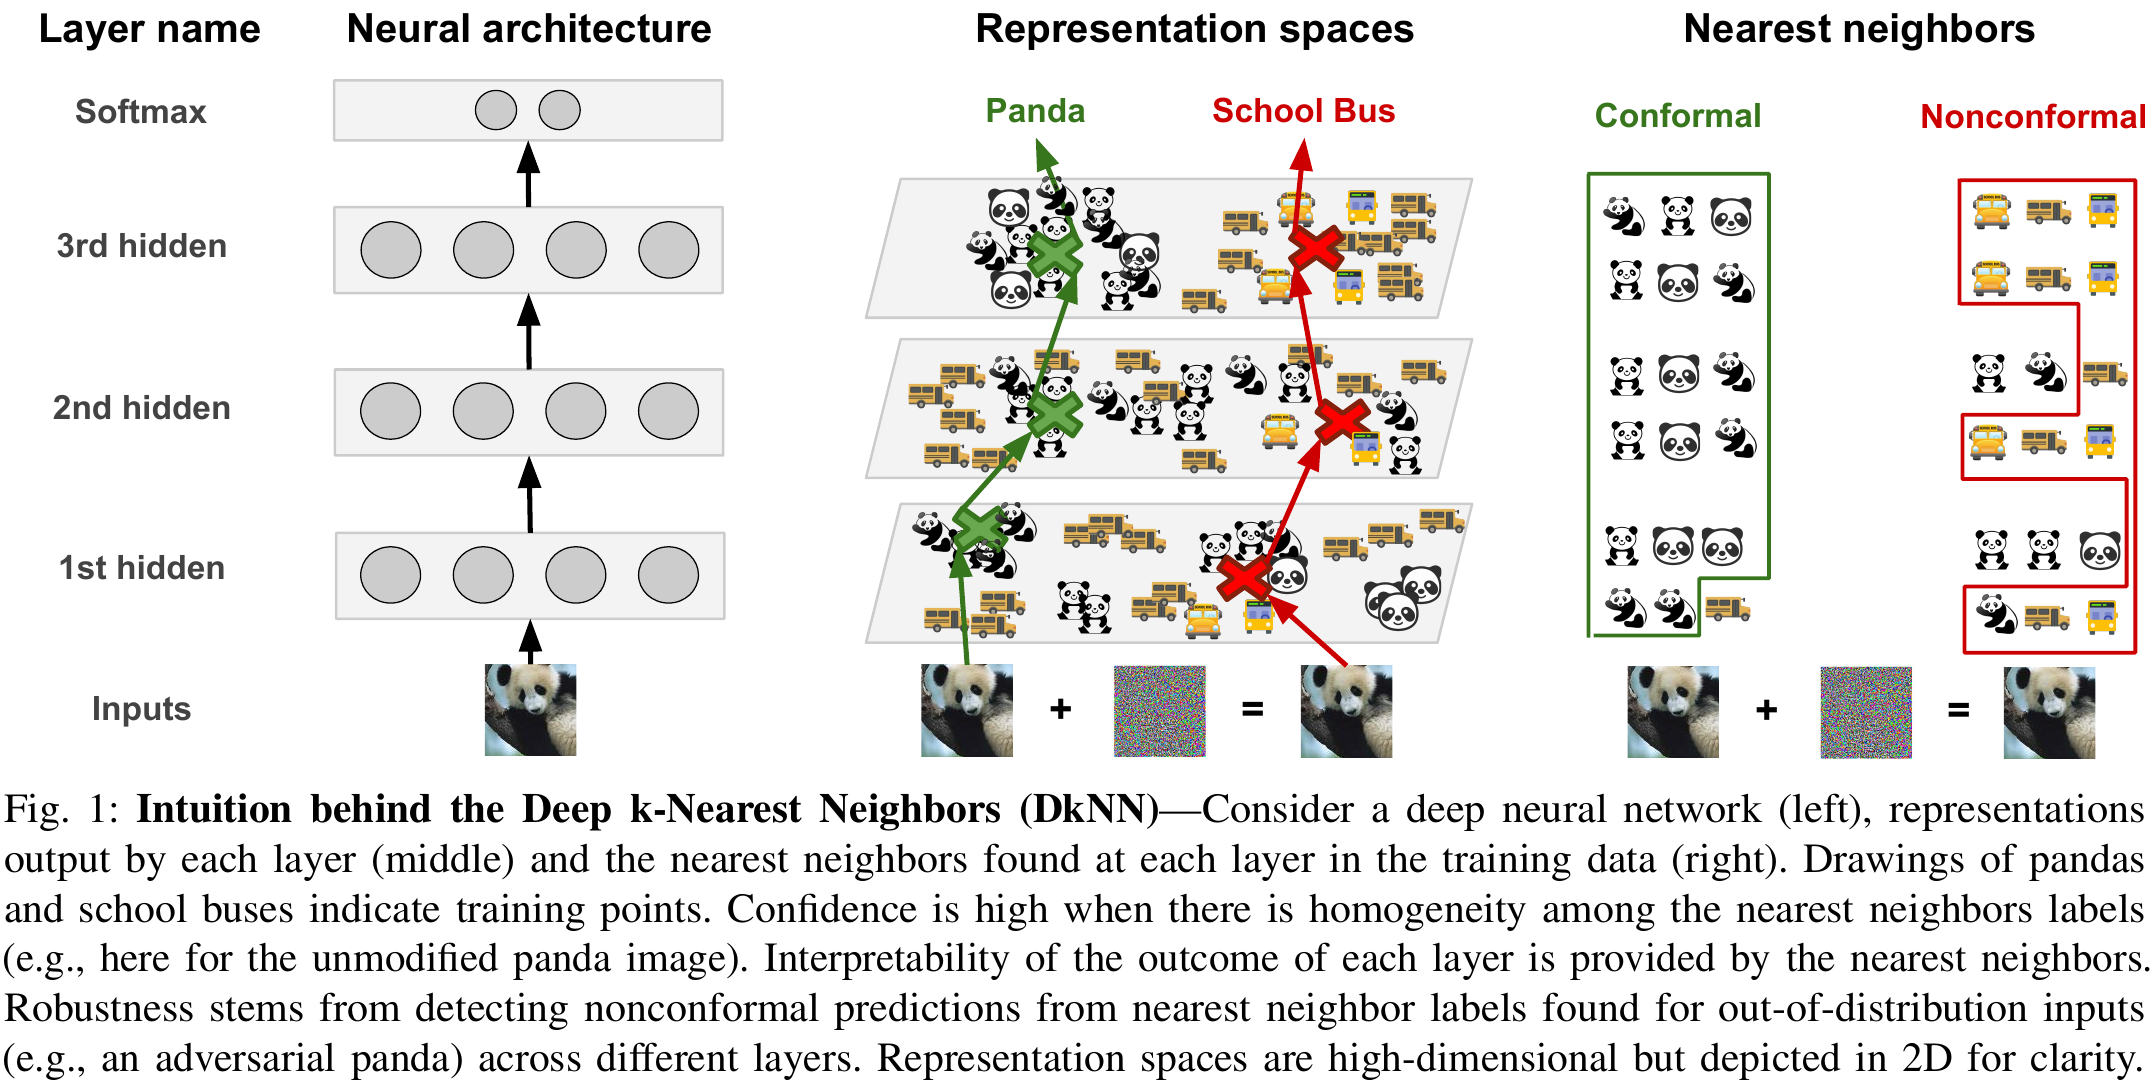
\includegraphics[width=\linewidth]{figures/papernot2018-figure1.png}
    \caption{Reproduced from Figure 1 of \citet{papernot2018deep}, including the original caption.}
    \label{fig:papernot-figure1}
\end{figure}

\clearpage 

\item \emph{(Question 3)}

\begin{itemize}
    \item The prior probabilities are:
    \[
    \begin{aligned}
        P(\text{Yes}) &= \frac{\text{Number of stolen vehicles}}{\text{Total number of vehicles}} = \frac{5}{10} = 0.500, \\
        P(\text{No}) &= \frac{\text{Number of non-stolen vehicles}}{\text{Total number of vehicles}} = \frac{5}{10} = 0.500.
    \end{aligned}
    \]
    \item Using the Naive-Bayes assumption, the conditional likelihoods are:
    \[
    \begin{aligned}
        P(\text{Red, Domestic, SUV} \mid \text{Yes})
        &= P(\text{Red} \mid \text{Yes})\,P(\text{Domestic} \mid \text{Yes})\,P(\text{SUV} \mid \text{Yes}) \\
        &= \frac{3}{5}\cdot\frac{2}{5}\cdot\frac{1}{5} = 0.048.
    \end{aligned}
    \]
    \[
    \begin{aligned}
        P(\text{Red, Domestic, SUV} \mid \text{No})
        &= P(\text{Red} \mid \text{No})\,P(\text{Domestic} \mid \text{No})\,P(\text{SUV} \mid \text{No}) \\
        &= \frac{2}{5}\cdot\frac{3}{5}\cdot\frac{3}{5} = 0.144.
    \end{aligned}
    \]
    \item The unnormalized posterior scores are:
    \[
    \begin{aligned}
        \text{Score(Yes)} &= P(\text{Yes})\,P(\text{Red, Domestic, SUV} \mid \text{Yes}) \\
        &= 0.500\cdot 0.048 = 0.024, \\
        \text{Score(No)} &= P(\text{No})\,P(\text{Red, Domestic, SUV} \mid \text{No}) \\
        &= 0.500\cdot 0.144 = 0.072.
    \end{aligned}
    \]
    Since $0.072 > 0.024$, the predicted class is No (not stolen).
    \item If a required conditional count were zero, the entire class score would become zero. If we fix this by applying Laplace smoothing, we would add 1 to every possible value's count, including nonzero counts, and then add the number of possible values of that feature to the denominator. 
    For example, since Type can be Sports or SUV, if the probability for Sports given Yes stolen was $\frac{0}{5}$ we would change the conditional likelihood to $\frac{0+1}{5+2}=\frac{1}{7}$. The conditional likelihoods for Color and Origin would also be shifted similarly.
\end{itemize}

\item \emph{(Question 4)} 

\item \emph{(Question 5)} Solutions to this problem were created with Codex GPT-6 Astra. A log of my conversation was maintained by Astra in the Markdown file labeled \path{q5_ai_conversation_log.md}. Most of my prompts
are recorded verbatim, but some longer ones have been summarized. I prompted Astra to write summaries of the work we did for this problem, but the reflection requested in Bullet Point 4 was written by me. 
% Student will add context and the final reflection separately.
\par\medskip
\noindent\textbf{Identified problems and corrections.}
The corrected notebook is \path{q5_corrected.ipynb}.
Line numbers refer to the original \path{q5_starter_classifier.py}.
The explanations and notebook evidence below were prepared with AI assistance;
independent validation is recorded separately in the AI-use conversation log.

\begin{enumerate}[label=\alph*.]
    \item \textbf{CSV headers are parsed as numeric data (line 27).}
    The original \texttt{np.loadtxt} call does not skip the header row
    \texttt{F1,F2,F3,F4,Class}. It therefore fails while converting
    \texttt{F1} to a floating-point number, before any model can run.
    The correction skips the single header row:
\begin{lstlisting}
np.loadtxt(path, delimiter=",", skiprows=1)
\end{lstlisting}
    \textbf{Evidence:} Figure~\ref{fig:q5-csv-header-error} shows the original
    loading failure. The corrected notebook successfully loads 910 training
    rows and 462 test rows, each with five numeric columns. Thus the correction
    resolves an execution failure rather than merely changing formatting.

    \item \textbf{The distance function sums signed differences (lines 30--31).}
    The expression \texttt{np.sum(a - b)} is not Euclidean distance:
    differences can cancel, and the result can be negative.
    In addition, $\sum_j(q_j-r_j)=\sum_j q_j-\sum_j r_j$, so sorting these
    scores favors training rows with larger coordinate sums independently
    of the query, apart from numerical tie effects.
    The corrected function computes the square root of the sum of squared
    coordinate differences:
\begin{lstlisting}
return np.sqrt(np.sum((a - b) ** 2))
\end{lstlisting}
    \textbf{Evidence:} For $(0,0)$ and $(3,4)$, the original result is
    $-7.000$, whereas the corrected distance is $5.000$. For $(0,0)$ and
    $(3,-3)$, the original result is $0.000$, whereas the corrected result is
    $\sqrt{18}\approx4.243$. These examples demonstrate both a failure of
    the original formula and agreement of the correction with Euclidean geometry.

    \item \textbf{Class values are included in feature coordinates (lines 50--54).}
    The starter scales all five columns into \texttt{train\_x} and
    \texttt{test\_x}, including the final class column. Extracting labels
    afterward does not remove that column from the feature arrays. This exposes
    the true test labels to the predictor and makes the feature representation
    invalid for evaluating classification.
    The correction separates features and labels before preprocessing:
\begin{lstlisting}
X_train = train[:, :-1]
y_train = train[:, -1].astype(int)
X_test = test[:, :-1]
y_test = test[:, -1].astype(int)
\end{lstlisting}
    Only the four-column feature arrays are scaled and passed to the distance
    calculation; labels remain separate for voting and evaluation.
    \textbf{Evidence:} The original transformations preserve all five columns.
    The corrected notebook reports feature shapes $(910,4)$ and $(462,4)$.
    The slices explicitly exclude the last column while preserving its values
    in the separate label arrays.

    \item \textbf{Scaling is fitted using test data (line 50).}
    The starter combines training and test rows before fitting its scaler, so test
    values influence the means and standard deviations used to prepare the
    model inputs. This is preprocessing leakage and compromises the held-out
    evaluation, whether or not it increases measured accuracy.
    The correction fits on training features alone and reuses those parameters:
\begin{lstlisting}
scaler = StandardScaler().fit(X_train)
train_scaled = scaler.transform(X_train)
test_scaled = scaler.transform(X_test)
\end{lstlisting}
    The internal training/validation split likewise fits its scaler only on the
    fitting subset.
    \textbf{Evidence:} The pooled F2 mean is $1.922$, while the training-only
    F2 mean is $2.010$, demonstrating that test data alter the original fitted
    parameters. The corrected notebook verifies that the scaler's mean vector
    equals the training-feature mean vector.

    \item \textbf{Vote ties silently favor class 0 (line 38).}
    The starter counts votes by class and selects the index with the largest
    count using \texttt{argmax}. For equal binary class
    counts, \texttt{argmax} selects index 0. The corrected notebook instead
    adopts Question 1's stated policy: choose the label of the nearest neighbor
    whose class is tied for the most votes. This is a voting-policy alignment
    with Q1; Q5 does not independently prescribe a particular tie policy.
\begin{lstlisting}
classes, counts = np.unique(votes, return_counts=True)
tied = classes[counts == counts.max()]
return next(label for label in votes if label in tied)
\end{lstlisting}
    Here \texttt{votes} is ordered by increasing neighbor distance.
    \textbf{Evidence:} Nearest-first votes $[1,0,1,0]$ yield counts $[2,2]$,
    so the starter chooses 0 while the adopted policy chooses 1. The notebook's
    four-neighbor toy example confirms that a tied vote returns the nearest
    neighbor's class, 1.
\end{enumerate}

\begin{figure}[htbp]
    \centering
    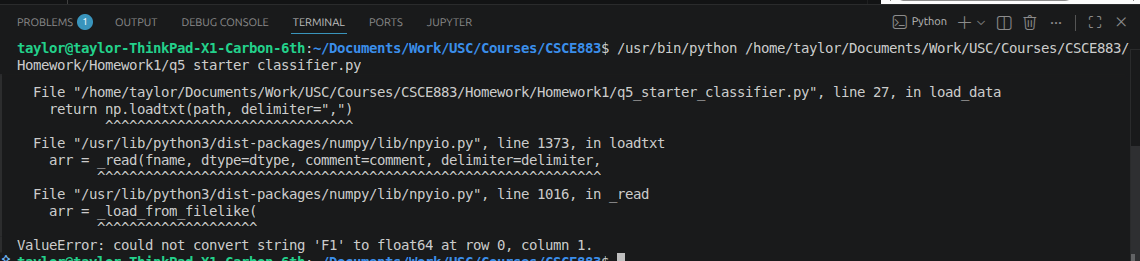
\includegraphics[width=\linewidth]{figures/q5-csv-header-error.png}
    \caption{Q5 starter CSV-loading error: line 27 attempts to convert the column header \texttt{F1} to a floating-point number.}
    \label{fig:q5-csv-header-error}
\end{figure}

% Parenthetical citations: \citep{papernot2018deep} or \citep{bergman2020deep}.
% Author-in-text citations: \citet{papernot2018deep} or \citet{bergman2020deep}.
\end{enumerate}

% Include both selected papers before citations are added to the report.
\nocite{papernot2018deep,bergman2020deep}
\bibliographystyle{plainnat}
\bibliography{references}

\end{document}

% Quick aligned table for equations and explanations
%
%\begin{center}
%  \begin{tabular}{l l l l}
%    % template line 
%    % LHS & $=$ & RHS & \emph{(comment)}\\
%   \end{tabular}
% \end{center}
